\maketitle
\tableofcontents
\newpage

\section{Zielsetzung}
Gegenstand des Versuches ist der Lock-In-Verstärker, dessen Funktionsweise
erforscht werden soll.

\section{Theorie}
\label{sec:2}
Der Lock-In-Verstärker wird überwiegend bei Messungen mit stark verrauschten Signalen
verwendet, um die gesuchte Frequenz herauszufiltern, ähnlich wie mit einem Bandpass.
Die Güte des Lock-In-Verstärkers liegt allerdings etwa um den Faktor 100 höher als
der eines Bandpasses.

Die Funktionsweise eines Lock-In-Verstärkers liegt darin,
die Messsignal mit einer Referenzfrequenz $\omega_0$ zu modulieren. In diesem Zuge
werden das Nutzsignal $U_ {sig}$ und das Referenzsignal $U_{ref}$ in einem Mischer
miteinander multipliziert\footnote{Näheres zum Aufbau in Kapitel \ref{sec:3.1}}
und anschließend als Mischsignal $U_{sig} \times U_{ref}$ über mehrere Perioden
der Modulationsfrequenz integriert, sodass sich die unerwünschten Rauschbeiträge
weitgehend herausmitteln und am Ausgang eine Gleichspannung $U_{out} \propto U_{sig} \,
\symup{cos}(\phi)$ zu messen ist, die sich proportional zu $U_{sig}$ verhält. Dabei
ist $\phi$ die veränderliche Phasenlage des Referenzsignals, die mit dem Nutzsignal synchronisiert
wird.

\begin{figure}
  \centering
  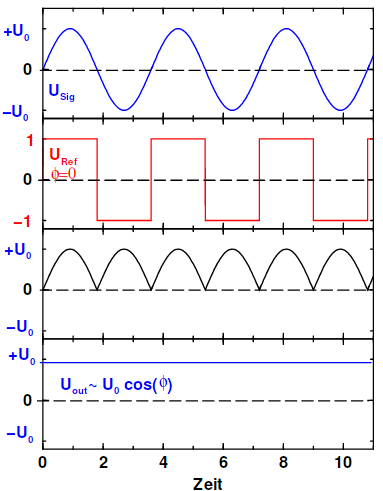
\includegraphics[scale=0.4]{theorie.png}
  \caption{Spannungsverläufe für eine sinusförmige Nutzspannung.}
  \label{fig:1}
\end{figure}
In Abbildung \ref{fig:1} wird der Signalverlauf für eine sinusförmiges Nutzspannung
\begin{equation*}
    U_{sig} = U_0 \, \symup{sin}(\omega \, t)
\end{equation*}
dargestellt. $U_{ref}$ ist hierbei durch eine Rechteckspannung mit gleicher Frequenz
moduliert. Wenn man Diese nun durch eine Fourierreihe nähert, enthält das Produkt
aus Nutz- und Referenzsignal $U_{sig} \times U_{ref}$ also nur die geraden Oberwellen
der Grundfrequenz $\omega$. % Hier eventuell die Gleichungen einfügen?
Der nachgeschaltete Tiefpassfilter unterdrückt nun diese Oberwellen. Damit erhält
man eine Gleichspannung der Form
\begin{equation}
    U_{out} = \frac{2}{\pi} \, U_0
    \label{eqn:4}
\end{equation}
Mit einer Phasendifferenz $\phi$ zwischen Nutz- und Referenzspannung wird
\eqref{eqn:4} zu
\begin{equation}
  U_{out} = \frac{2}{\pi} \, U_0 \, \symup{cos}(\phi) \ .
  \label{eqn:5}
\end{equation}
Die Ausgangsspannung wird also maximal für $\phi = 0$, also wenn es keinen Phasenunterschied
zwischen Nutz- und Referenzspannung gibt.

\section{Durchführung}
\subsection{Versuchsaufbau}
\label{sec:3.1}
\begin{figure}
  \centering
  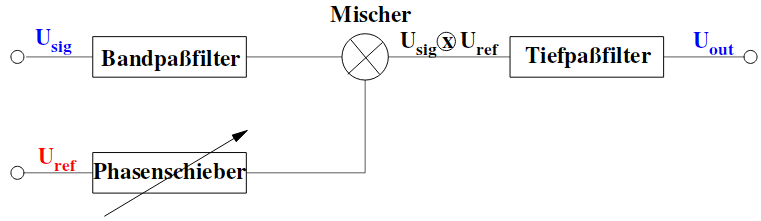
\includegraphics[scale=0.4]{aufbau.png}
  \caption{Schematischer Aufbau eines Lock-In-Verstärkers.}
  \label{fig:2}
\end{figure}
Wie in Abbildung \ref{fig:2} zu sehen, wird $U_{sig}$ mithilfe eines Bandpasses
von Rauschanteilen höherer und niedriger Frequenzen gereinigt. Als nächstes kommt
der bereits erwähnte Mischer\footnote{siehe Kapitel \ref{sec:2}}, der Nutz- und
Referenzsignal miteinander multipliziert, wobei sich die Phase des Referenzsignals
mit dem Phasenschieber einstellen lässt. Nachgeschaltet dazu gibt es noch einen
Tiefpass, dessen Funktion bereits in Kapitel \ref{sec:2} erläutert wurde. Zum
Schluss erhält man das Ausgangssignal $U_ {out}$.

\subsection{Versuchsdurchführung}
\begin{figure}
  \centering
  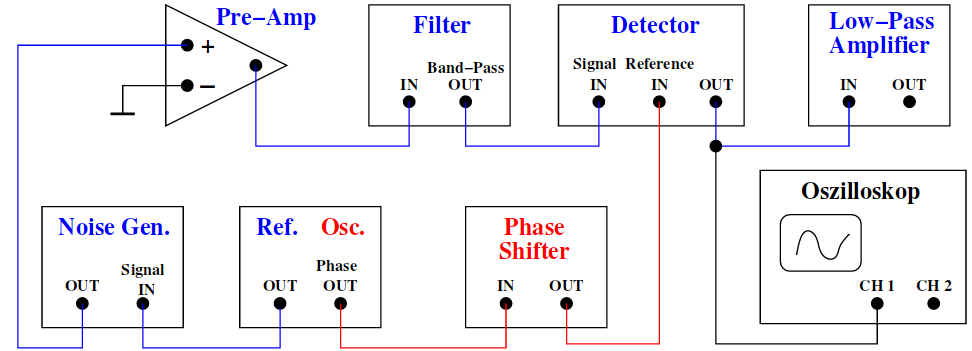
\includegraphics[scale=0.3]{durch.png}
  \caption{Schaltplan eines Lock-In-Verstärkers.}
  \label{fig:3}
\end{figure}
Als erstes wurde festgestellt, welcher Ausgang der Funktionsgenerators in Abbildung
\ref{fig:3} eine variable und welcher eine konstante Spannung liefert, und welchen
Wert Diese hat. Danach wurde der Schaltplan Schritt für Schritt aufgebaut und dabei
auf einem Speicher-Oszilloskop die Signalformen überprüft und mithilfe der Print-Funktion
Skizzen des Signals nach jedem Schritt gemacht. Dabei wird der Noise-Generator
zwar eingebunden, aber noch nicht eingeschaltet, um zuerst Messungen ohne Rauschsignal
aufzunehmen. Als nächstes wird ein sinusförmiges Signal $U_{sig}$ von % Hier brauche ich die Werte aus dem Buch
$\SI{1}{\kilo\hertz}$ und $\SI{0.01}{\volt}$ erzeugt und mit einem Referenzsignal
$U_{ref}$, welches auch sinusförmig ist und die gleiche Frequenz hat, gemischt.
Nach der Integration über den Tiefpass wird die Ausgangsspannung $U_{out}$ % Hier auch die richtige Zahl
zehnmal in Abhängigkeit von der Phasenverschiebung bestimmt.

Anschließend wird der Noise-Generator eingeschaltet und alle Messungen wiederholt.
Dabei liegt die Größenordnung des Rauschsignals ungefähr in der Größenordnung
von $U_{sig}$.

\begin{figure}
  \centering
  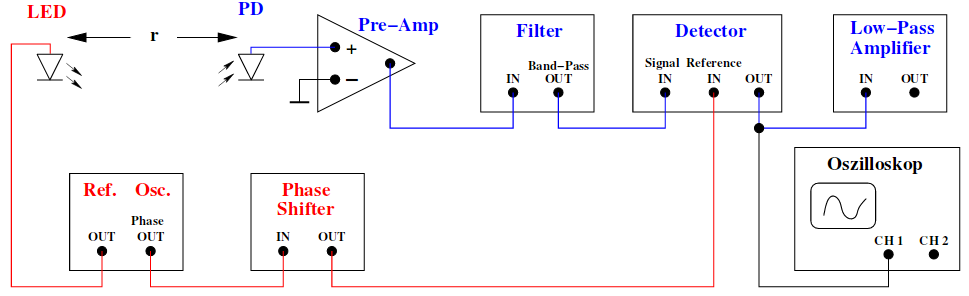
\includegraphics[scale=0.3]{durch2.png}
  \caption{Schaltplan eines Lock-In-Verstärkers mit Photo-Detektor.}
  \label{fig:4}
\end{figure}
Als letztes wird ein Photo-Detektor in den Schaltplan eingefügt\footnote{siehe Abbildung \ref{fig:4}},
dessen LED mit $\SI{200}{\hertz}$ % Hier auch richtiger Wert
blinkt und mit einer Rechteckspannung moduliert wird. Dann wird die Lichtintensität
als Funktion des Abstandes zwischen LED und Photodiode gemessen und der maximale
Abstand $r_{max}$ bestimmt, bei dem das Licht der LED die Photodiode nachweislich
noch erreicht.

% \section{Fehlerrechnung}
% Es gibt:
% \begin{equation}
%   \bar{T} = \frac{1}{n} \sum_{i=1}^{n} T_{i}
%   \label{eqn:1}
% \end{equation}
% den Mittelwert und:
% \begin{equation}
%   \sigma_{\bar{T}} = \sqrt{\frac{1}{n(n-1)} \sum_{i=1}^{n}(\bar{T}-T_i)^2}
%   \label{eqn:2}
% \end{equation}
% den Fehler des Mittelwertes. Falls zwei fehlerbehaftete Größen in einer Gleichung
% zur Bestimmung einer anderen Größe Verwendung finden, dann berechnte sich der Gesamtfehler
% nach der Gaußschen Fehlerfortpflanzung zu
% \begin{equation}
%     \symup \Delta f(x_1, x_2, ..., x_n) = \sqrt{\left(\frac{\symup df}{\symup dx_1} \symup \Delta
%     x_1 \right)^2 +    \left(\frac{\symup df}{\symup dx_2} \symup \Delta
%     x_2 \right)^2 + ... + \left(\frac{\symup df}{\symup dx_n} \symup \Delta x_n \right)^2} \ .
%     \label{eqn:3}
% \end{equation}

\section{Auswertung}
\subsection{Verwendung des Lock-In Verstärkers mit und ohne künstlichem Rauschen}
\begin{table}
  \centering
  \caption{Mit Gain von 5 gemessene Werte}
  \label{tab:1}
  \begin{tabular}{c c c}
    \toprule
    Phase/$\si{\pi}$ & $U_{unverauscht}/\si{\volt}$ & $U_{verauscht}/\si{\volt}$ \\
    \midrule
    0.00 & 6.00 & 6.00 \\
    0.17 & 5.00 & 5.00 \\
    0.25 & 3.50 & 3.50 \\
    0.33 & 1.50 & 1.50 \\
    0.50 & -1.00 & -1.00 \\
    0.67 & -3.50 & -3.50 \\
    0.75 & -5.00 & -5.00 \\
    0.83 & -6.00 & -6.00 \\
    1.00 & -6.00 & -6.00 \\
    1.25 & -3.50 & -3.50 \\
    1.50 & 1.00 & 1.00 \\
    1.83 & 6.00 & 6.00 \\
    \bottomrule
  \end{tabular}
\end{table}
\begin{figure}
  \centering
     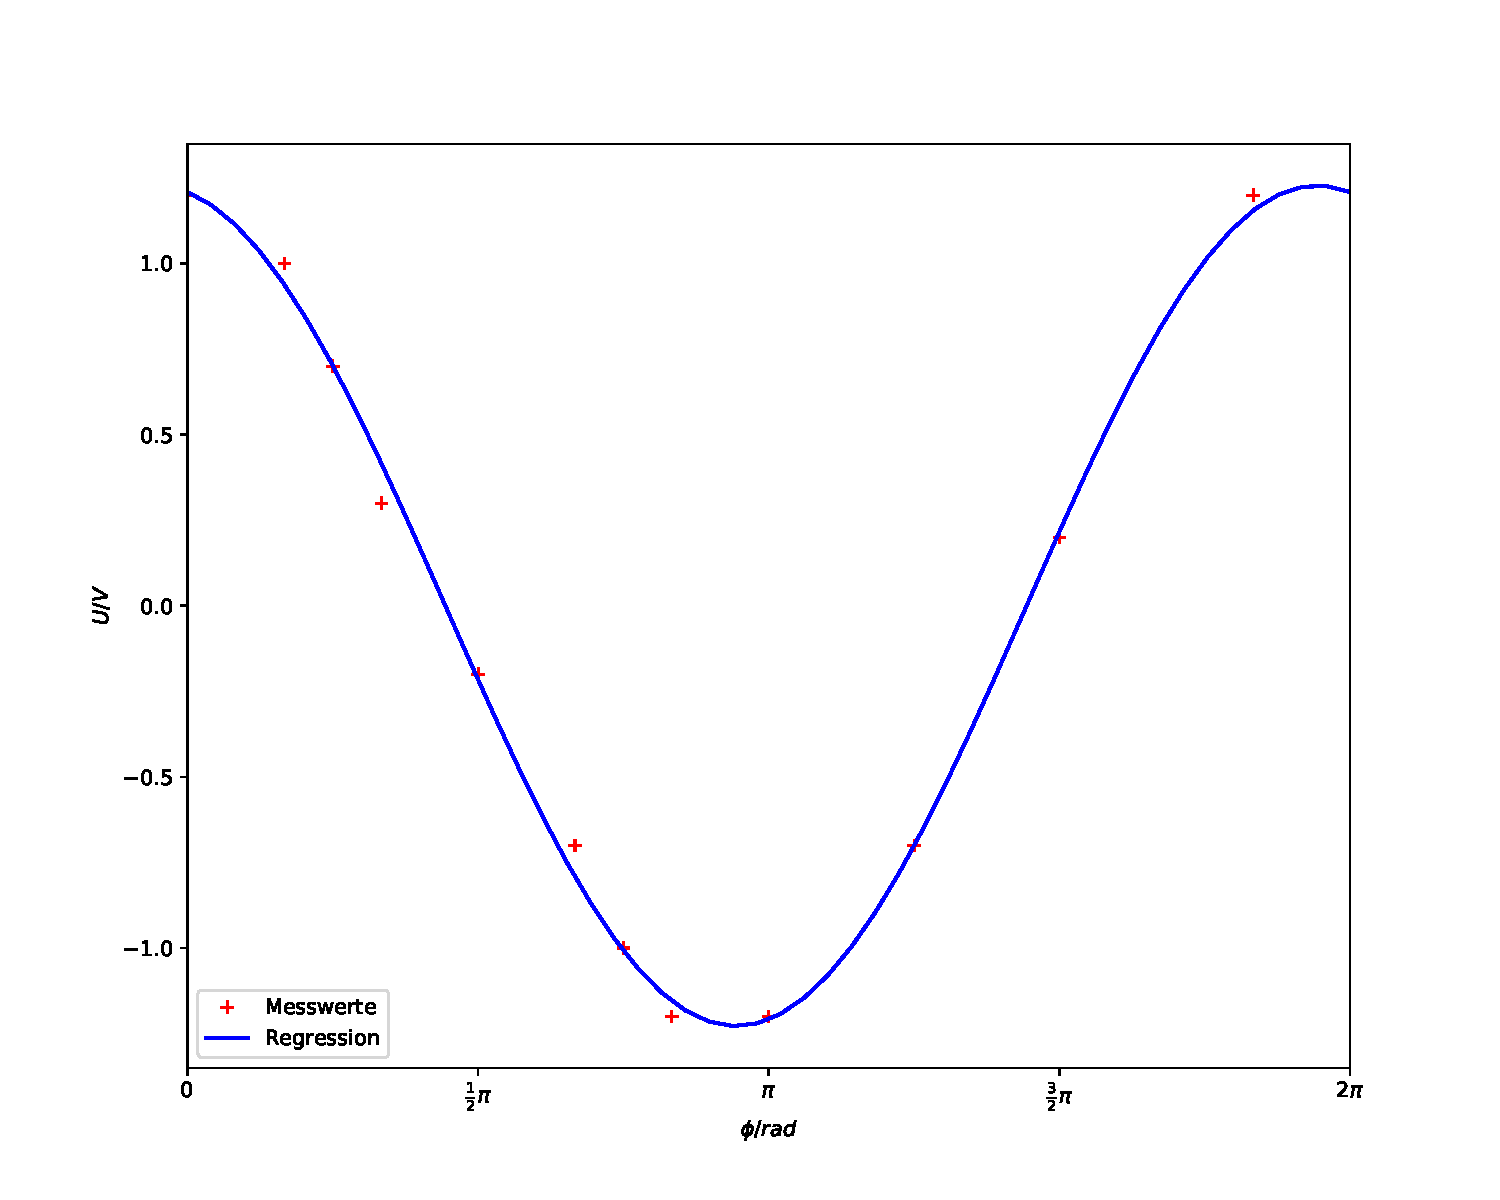
\includegraphics[scale=0.6]{UvonPhi.pdf}
  \caption{Auftragen der gemessenen Spannungen gegen die Phasen mit Regression. Die Spannungen sind vom Verstärkungsfaktor bereinigt.}
  \label{plot:1}
\end{figure}
Die am Tiefpassfilter mit und ohne Rauschen gemessenen Spannungen sind in Tabelle \ref{tab:1}
dargestellt. Es zeigt sich kein messbarer Unterschied zwischen unverrauschter und verrauschter Messung,
woraus auf die Ordnungsgemäße Funktionsweise des Aufbaus geschlossen werden kann.
Die Messwerte wurden bei einem Verstärkungsfaktor von 5 gemessen. Wird die Phase gegen die Spannung
aufgetragen, ergibt sich der in Grafik \ref{plot:1} dargestellte Verlauf. Werden die Messwerte mit einer
Funktion:
\begin{equation*}
  U_{out}(\phi) = A_0 \cdot \symup{cos}(\phi + \symup{\delta}\phi)
\end{equation*}
gefittet, wobei $A_0$ die Amplitude und $\symup{\delta}\phi$ die interne Phase des Aufbaus darstellt,
ergeben sich folgende Werte für Amplitude und Phase:
\begin{equation*}
  \begin{split}
    A_0 = \SI{1.228(22)}{\volt} \\
    \symup{\delta}\phi = \SI{0.177(19)}{\pi}
  \end{split}
\end{equation*}
Die gemessenen Werte folgen also dem nach \eqref{eqn:5} zu erwartenen Verlauf.
\subsection{Abstandsmessung}
\label{chapter:Abst}
\begin{table}
  \centering
  \caption{Mit Gain von 5 gemessene Werte}
  \label{tab:2}
  \begin{tabular}{c c}
    \toprule
    Abstand r/$\si{\centi\metre}$ & $U(r)/\si{\volt}$\\
    \midrule
    10 & 6.00 \\
    12 & 5.50 \\
    16 & 4.75 \\
    20 & 3.00 \\
    24 & 2.00 \\
    28 & 1.25 \\
    32 & 1.00 \\
    36 & 0.75 \\
    40 & 0.50 \\
    44 & 0.50 \\
    48 & 0.50 \\
    52 & 0.50 \\
    56 & 0.50 \\
    60 & 0 \\
    \bottomrule
  \end{tabular}
\end{table}
\begin{figure}
  \centering
     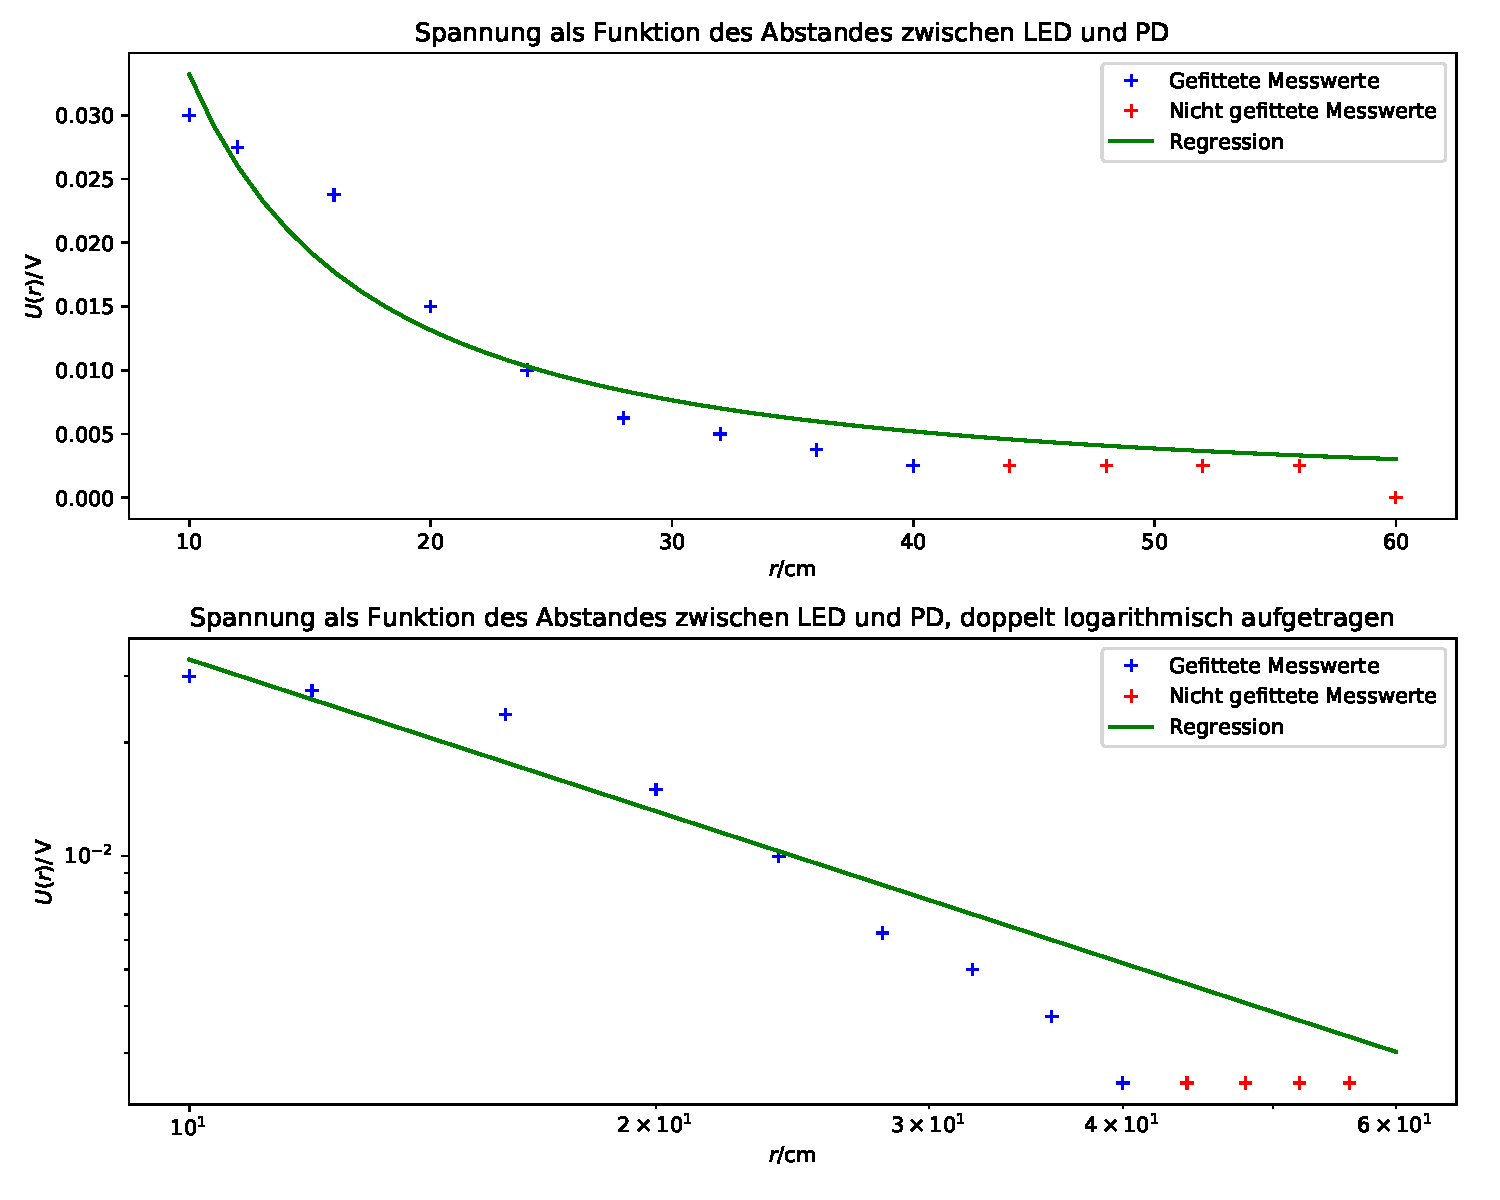
\includegraphics[scale=0.6]{SubABst.pdf}
  \caption{Auftragen der gemessenen Spannungen gegen den Abstand mit Regression. Die bei der Regression nicht
  beachteten Messwerte sind kenntlich gemacht.
  Die Spannungen sind vom Verstärkungsfaktor bereinigt. Der obere Verlauf ergibt sich bei normaler Achsenskalierung,
  der untere bei doppelt logarithmischer.}
  \label{plot:2}
\end{figure}
Wird der Abstand zwischen LED und Photodiode vergrößert, so ist ein Abfall der gemessenen Spannung $\propto 1/r^a$ zu erwarten.
Das Signal wurde dabei mit einer Frequenz von \SI{300}{\hertz} eingestellt, um die von den im Raum
befindlichen, mit einer Netzfrequenz von \SI{50}{\hertz} betriebenen, künstlichen Lichtquellen erzeugten
Störsignale nicht zusätzlich zu verstärken. Die bei einem Gain von 200 gemessenen Daten
(siehe Tabelle \ref{tab:2}) werden daher mit einer Funktion:
\begin{equation}
  U(r) = \frac{b}{r^a}
\end{equation}
gefittet. Die wiederholt auftretenden Messwerte von \SI{0.5}{\volt} werden, wie auch der Nullpunkt der Messung bei ca. \SI{60}{\centi\metre}
weggelassen. Dies ist vertretbar, da davon auszugehen ist, dass die zur Verfügung stehenden Messgeräte in diesem Bereich Änderungen nicht
mehr mit ausreichender Genauigkeit anzeigen können. Ein Gleichbleiben der Werte bei erhöhen des Abstandes
erscheint rein logisch unintuitiv und würde oben genannter Abstandsgesetzmäßigkeit wiedersprechen. Die Regression ist
in Grafik \ref{plot:2} in normaler sowie doppelt logarithmischer Achsenskalierung dargestellt.
Bei doppelt logarithmischer Skalierung zeigt sich ein linearer Verlauf, der bei einem Abstandsgesetz wie oben genannt
bei dieser Skalierung zu erwarten ist. Der Fit liefert:
\begin{equation*}
  \begin{split}
    a = \num{1.34(18)}\\
    b = \SI{0.72(34)}{\volt\square\centi\metre}
  \end{split}
\end{equation*}
Die Spannungen wurden vor dem Fit durch den Verstärkungswert geteilt. Der sinnvolle Verlauf der Messung
lässt wieder auf die Ordnungsgemäße Funktionsweise des Lock-In Verstärkers schließen.
\section{Diskussion}
Zusammenfassend belegt der Versuchsaufbau die gewünschte Funktionsweise des Lock-In Verstärkers. Insbesondere der erste Teil
des Versuchs zeigt dies sehr gut. Hier sind die Abweichungen zwischen verrauschter und unverrauschter Messung kaum mit
den zur Verfügung stehenden Geräten Messbar. Der zweiter Teil des Versuches hingegen liefert zwar
Werte, die auf den Nachweis des Abstandsgesetzes schließen lassen, jedoch, wie in Grafik \ref{plot:2} zu erkennen ist,
starke unregelmäßigkeiten Aufweisen. Hier sind definitiv erneute Messungen erforderlich, um
die ordnungsgemäße Funktionsweise des Lock-In Verstärkers zu zeigen.

Ansätze zur Verbesserung der Ergebnisse wären ein besseres Abstimmen der Verstärkungswerte, um ein
genaueres Ergebnis zu erhalten. Auch musste die Erfassung der Messwerte über ein analoges
Voltmeter mit großschrittiger Skala erfolgen. Ein digitales Gerät oder eine kleinschrittigere
Skala hätten die Güte der Messung hier erhöht. Insbesondere das in Kapitel \ref{chapter:Abst}
genannte gleichbleiben der Messwerte ab einem gewissen Punkt hätte durch ein genaueres
Messgerät verhindert werden können.\\
Auch eine Referenzmessung ohne Umgebungslicht wäre sinnvoll. Die dabei erhaltenen
Messwerte könnten für einen direkten Vergleich mit der Messung bei Umgebungslicht herangezogen werden.

\newpage
\nocite{*}
\printbibliography
